\documentclass{article}
\usepackage[utf8]{inputenc}
\usepackage{parskip}
\usepackage{graphicx}
\usepackage{float}

\title{Lab2 Machine Learning}
\author{Casper Renman\\casperr@kth.se \and Hampus Fristedt\\hamfri@kth.se}
\begin{document}
\maketitle

\section{Seed: 1625196557218803968, EZ-MODE, Class A mean=-2, std=1, Class B mean=2, std=1}
Fakking ez even linear can do this shit
\subsection{Linear}
\begin{figure}[H]
    \centering
    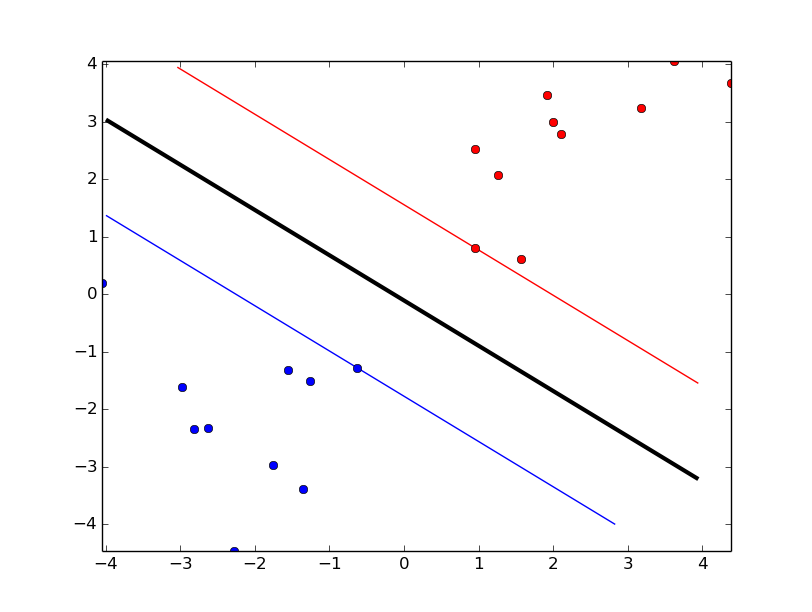
\includegraphics[width=1.0\linewidth]{../img/linear_s1_ez.png}
\end{figure}

\subsection{Polynomial}
p=2
\begin{figure}[H]
    \centering
    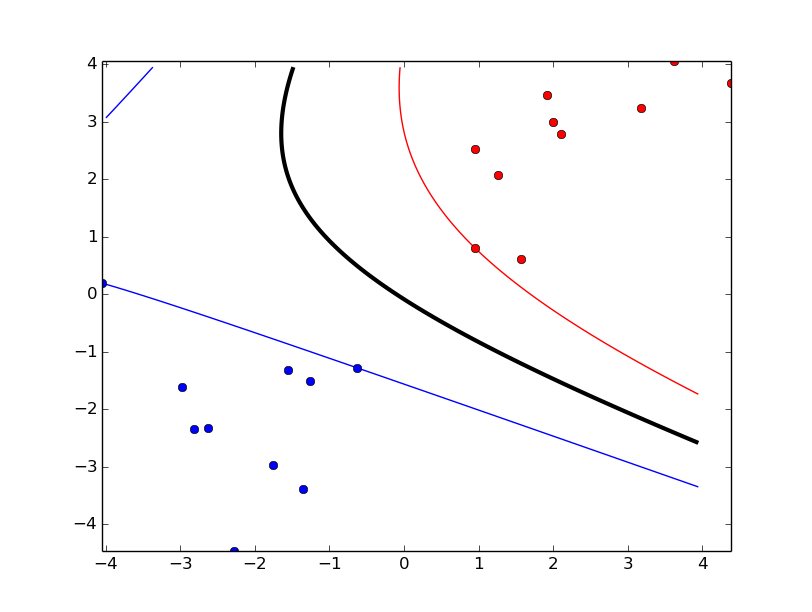
\includegraphics[width=1.0\linewidth]{../img/poly_s1_ez_p2.png}
\end{figure}

\subsection{Radial}
sigma=2
\begin{figure}[H]
    \centering
    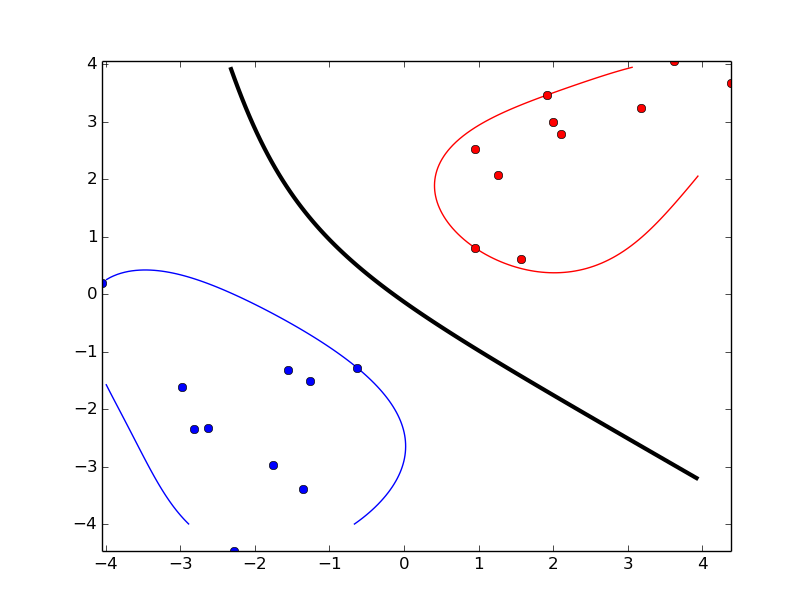
\includegraphics[width=1.0\linewidth]{../img/radial_s1_ez_s2.png}
\end{figure}

\section{Seed: 1625196557218803968, default values}
This is the default values given by the lab instructions.

\subsection{Linear}

\begin{figure}[H]
    \centering
    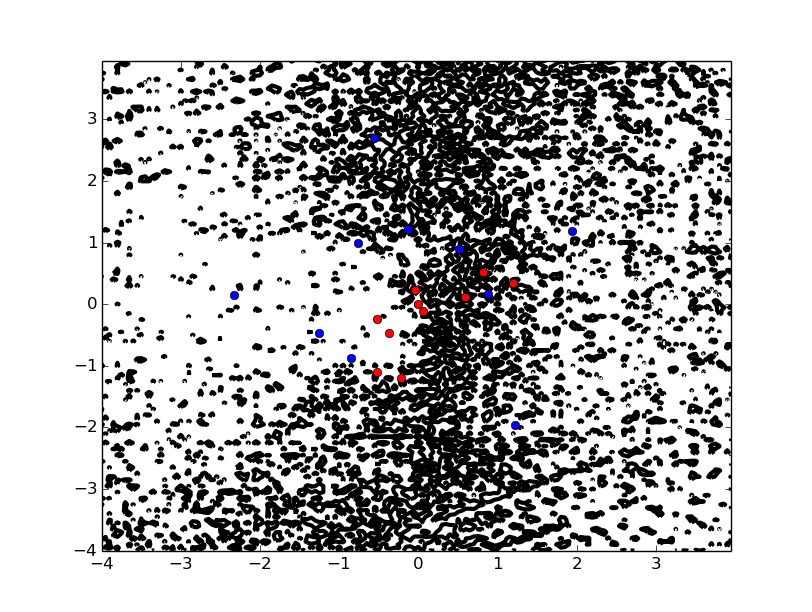
\includegraphics[width=1.0\linewidth]{../img/linear_s1.png}
\end{figure}

\subsection{Polynomial}

p = 2 resulted in no optimal solution.

p = 3
\begin{figure}[H]
    \centering
    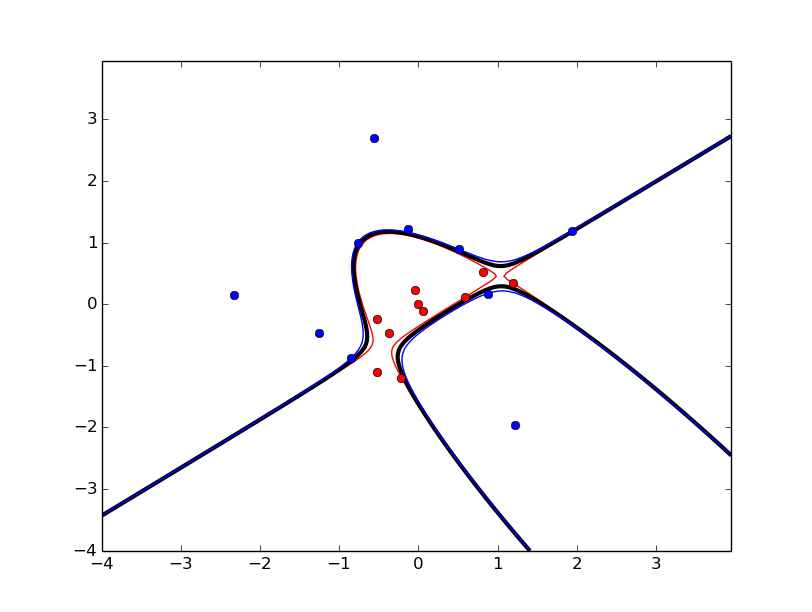
\includegraphics[width=1.0\linewidth]{../img/poly_s1_p3.png}
\end{figure}

p = 4
\begin{figure}[H]
    \centering
    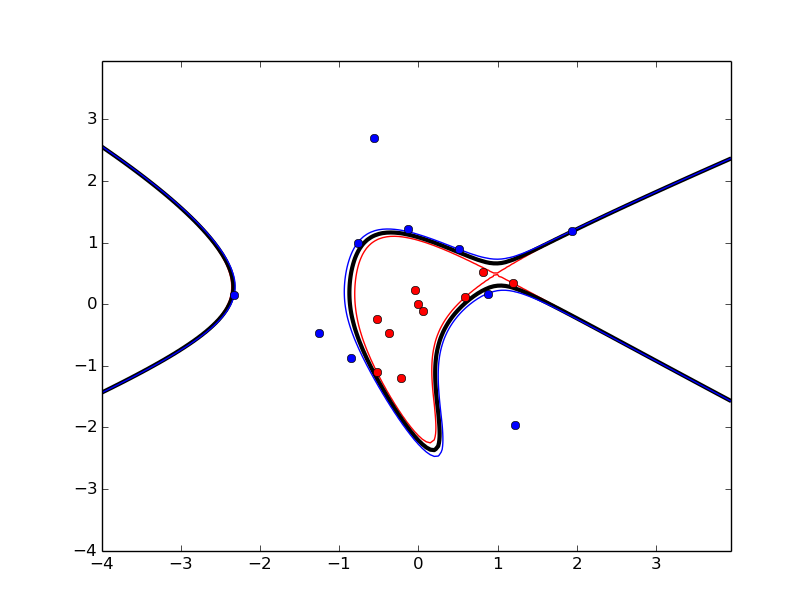
\includegraphics[width=1.0\linewidth]{../img/poly_s1_p4.png}
\end{figure}

p = 15
\begin{figure}[H]
    \centering
    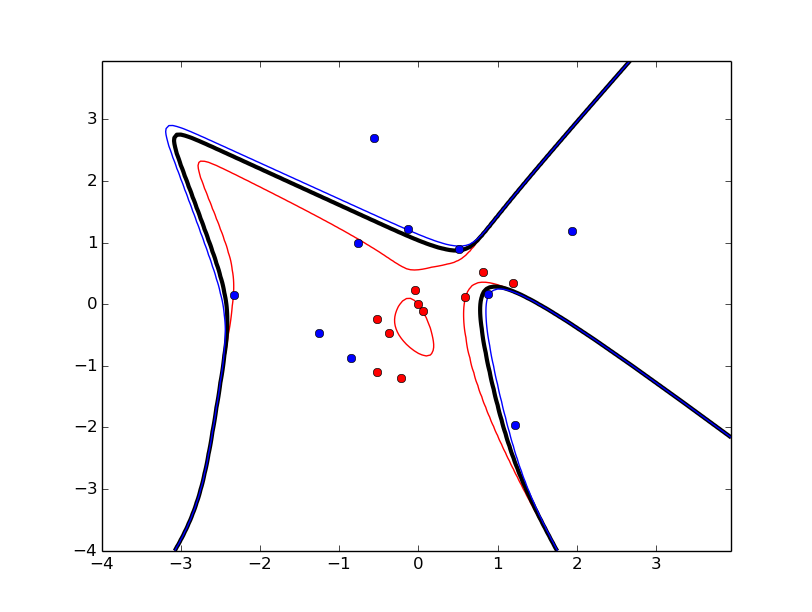
\includegraphics[width=1.0\linewidth]{../img/poly_s1_p15.png}
\end{figure}

\subsection{Radial}

s = 1
\begin{figure}[H]
    \centering
    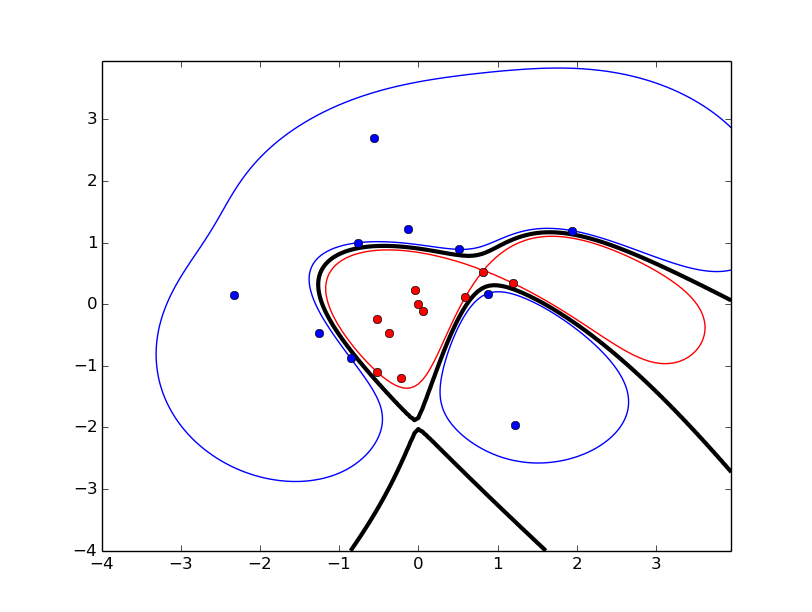
\includegraphics[width=1.0\linewidth]{../img/radial_s1_s1.png}
\end{figure}

s = 2
\begin{figure}[H]
    \centering
    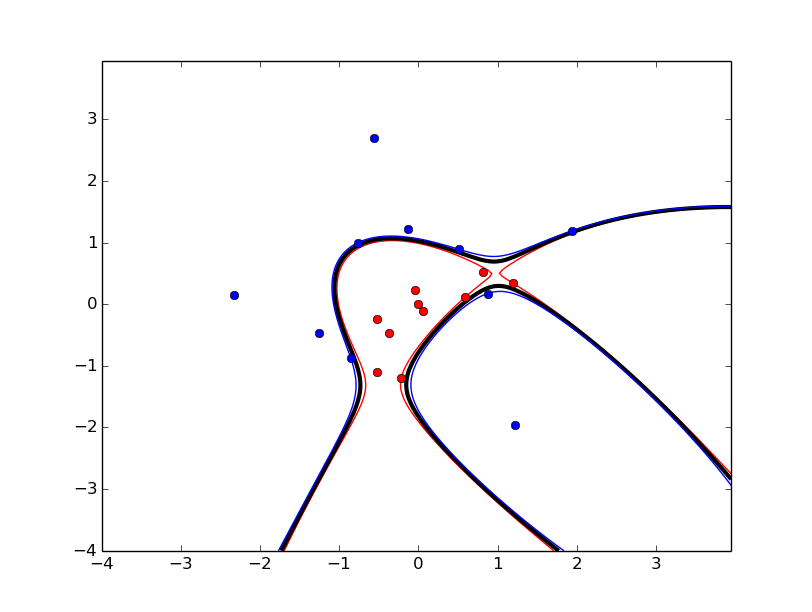
\includegraphics[width=1.0\linewidth]{../img/radial_s1_s2.png}
\end{figure}

s = 10
\begin{figure}[H]
    \centering
    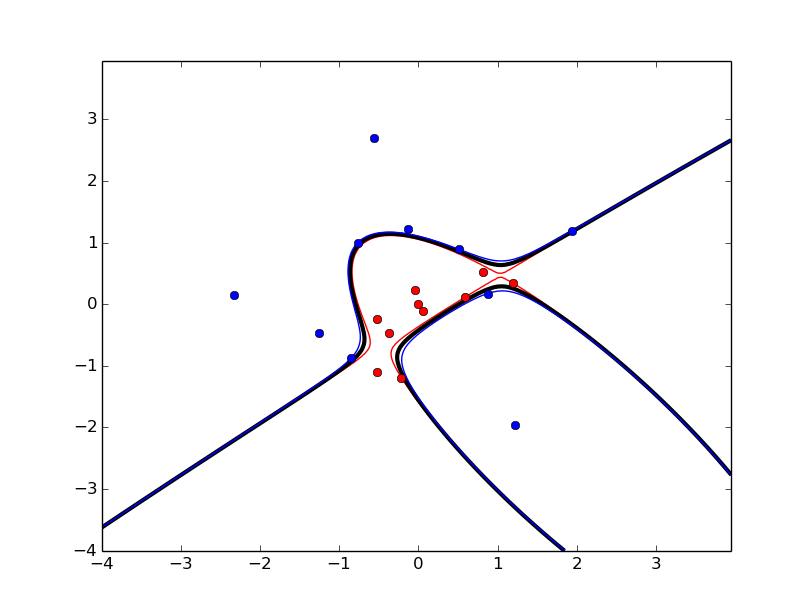
\includegraphics[width=1.0\linewidth]{../img/radial_s1_s10.png}
\end{figure}

\section{Seed: 1625196557218803968, no difference in position for class A and B, mean=origo, std=1}
\subsection{Linear}
The linear solver could not solve.

\subsection{Polynomial}
The polynomial solver could solve when $p=3$, but not earlier.

p = 3
\begin{figure}[H]
    \centering
    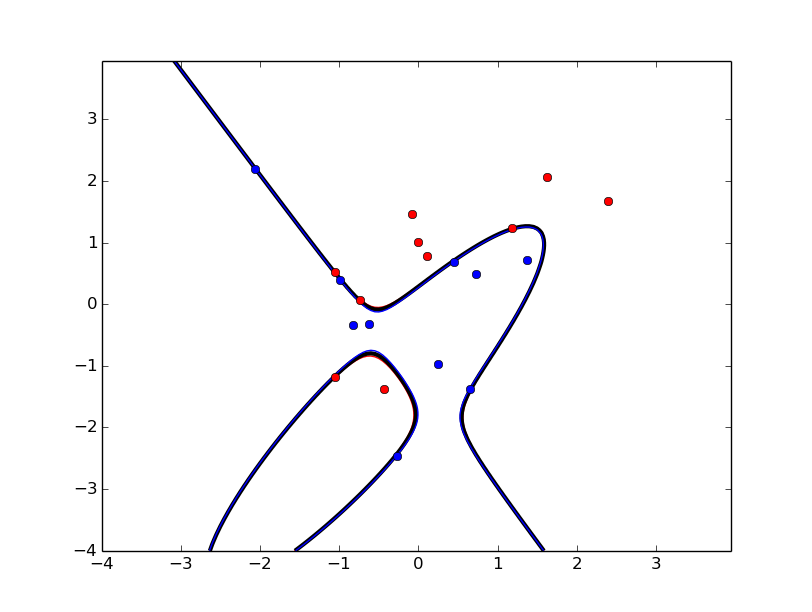
\includegraphics[width=1.0\linewidth]{../img/poly_s1_hard_p3.png}
\end{figure}

\subsection{Radial}
Radial is badass and can do anything.

s = 0.5 
\begin{figure}[H]
    \centering
    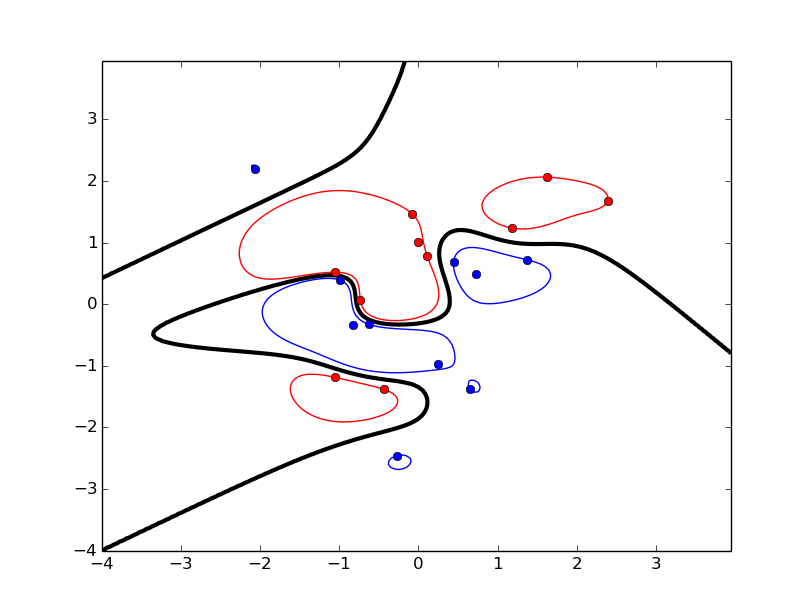
\includegraphics[width=1.0\linewidth]{../img/radial_s1_hard_s05.png}
\end{figure}

s = 1 
\begin{figure}[H]
    \centering
    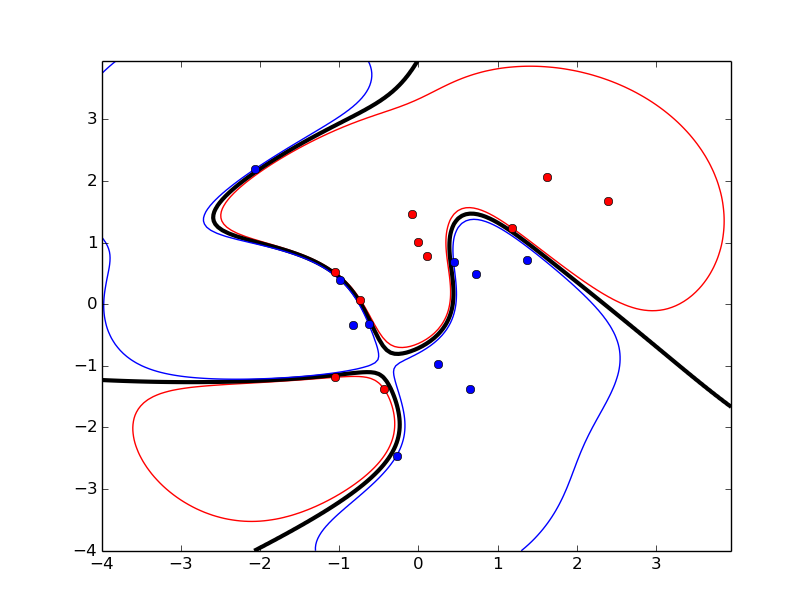
\includegraphics[width=1.0\linewidth]{../img/radial_s1_hard_s1.png}
\end{figure}

s = 2 
\begin{figure}[H]
    \centering
    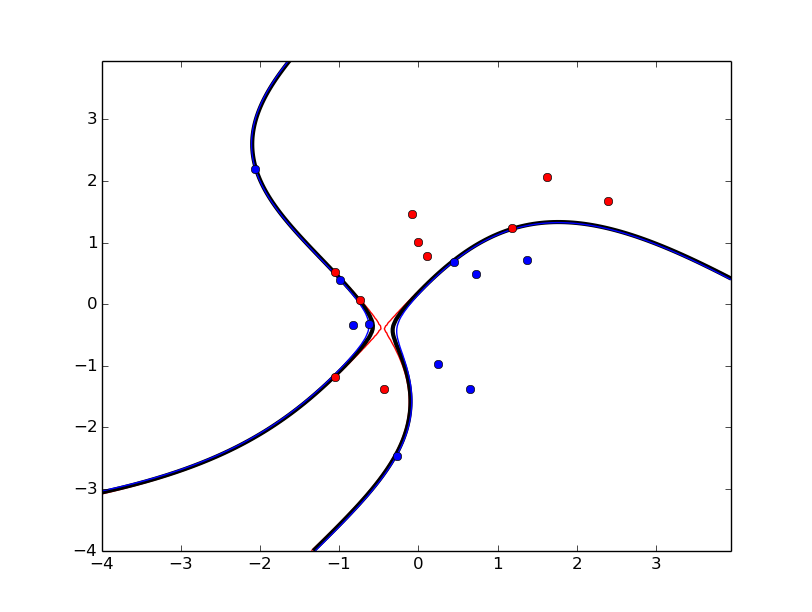
\includegraphics[width=1.0\linewidth]{../img/radial_s1_hard_s2.png}
\end{figure}

\end{document}
